%!TEX root = ../notas_de_clase.tex
\section{Support-vector machines}

Una de las desventajas de los clasificadores lineales vistos en el Capítulo \ref{cap:clasificacion} (en el caso binario) es la falta de atención al margen de las clases, es decir, la región entre las muestras de ambas clases, pues en esta región se encontrará el hiperplano de decisión. Esta distancia es relevante, pues nos da un sentido de generalización, es decir,  los elementos de la clase 1  \emph{más parecidos} a los de la clase -1 no están justo en el borde de las clases, sino que existe una zona donde podrían haber nuevas muestras en torno a datos existentes de clase, e.g., 1 y aún estar dentro de la región de clase 1. El tratamiento de este concepto (o la falta de él) es claro en los métodos anteriores: en el perceptrón, todas las soluciones que dividen las muestras clases $\pm 1$ son ``igual de buenas'', es decir, el perceptrón es insensible al margen descrito arriba. Por otro lado, para los métodos que funcionan mediante gradiente descendente como mínimos cuadrados o regresión logística, este margen se maximiza \emph{indirectamente}, lo cual conlleva a inestabilidades como en el caso en donde el parámetro de la regresión logística diverge. \\


Para resolver el problema descrito anteriormente consideraremos las \textbf{máquinas de soporte vectorial} (SVM, por sus siglas en inglés). Como veremos en este capítulo, además de resolver el problema de clasificación binaria y lineal, la solución de SVM puede ser ocupado en muchas más situaciones, por esta razón, dedicamos un capítulo completo a este método en vez de verlo como un método de clasificación más. 

\subsection{Idea general}

Consideremos un problema de clasificación donde las clases son linealmente separables. Como podemos ver en la Fig.~\ref{fig:maxim_marg} (izquierda), en este caso existen diferentes hiperplanos (clasificadores lineales) que separan los datos de ambas clases de forma correcta. Cada una de estas soluciones define un modelo, donde dado un nuevo dato $x_\star$, podemos evaluar a qué clase pertenece. Evidentemente, la asignación de clase usando cada uno de los clasificadores mostrados en la figura  anterior (izquierda) son similares en la mayoría del espacio salvo la región cercana al límite de las clases; es precisamente en este lugar donde nos enfocamos en este capítulo. 


\begin{figure}[ht]
    \centering
    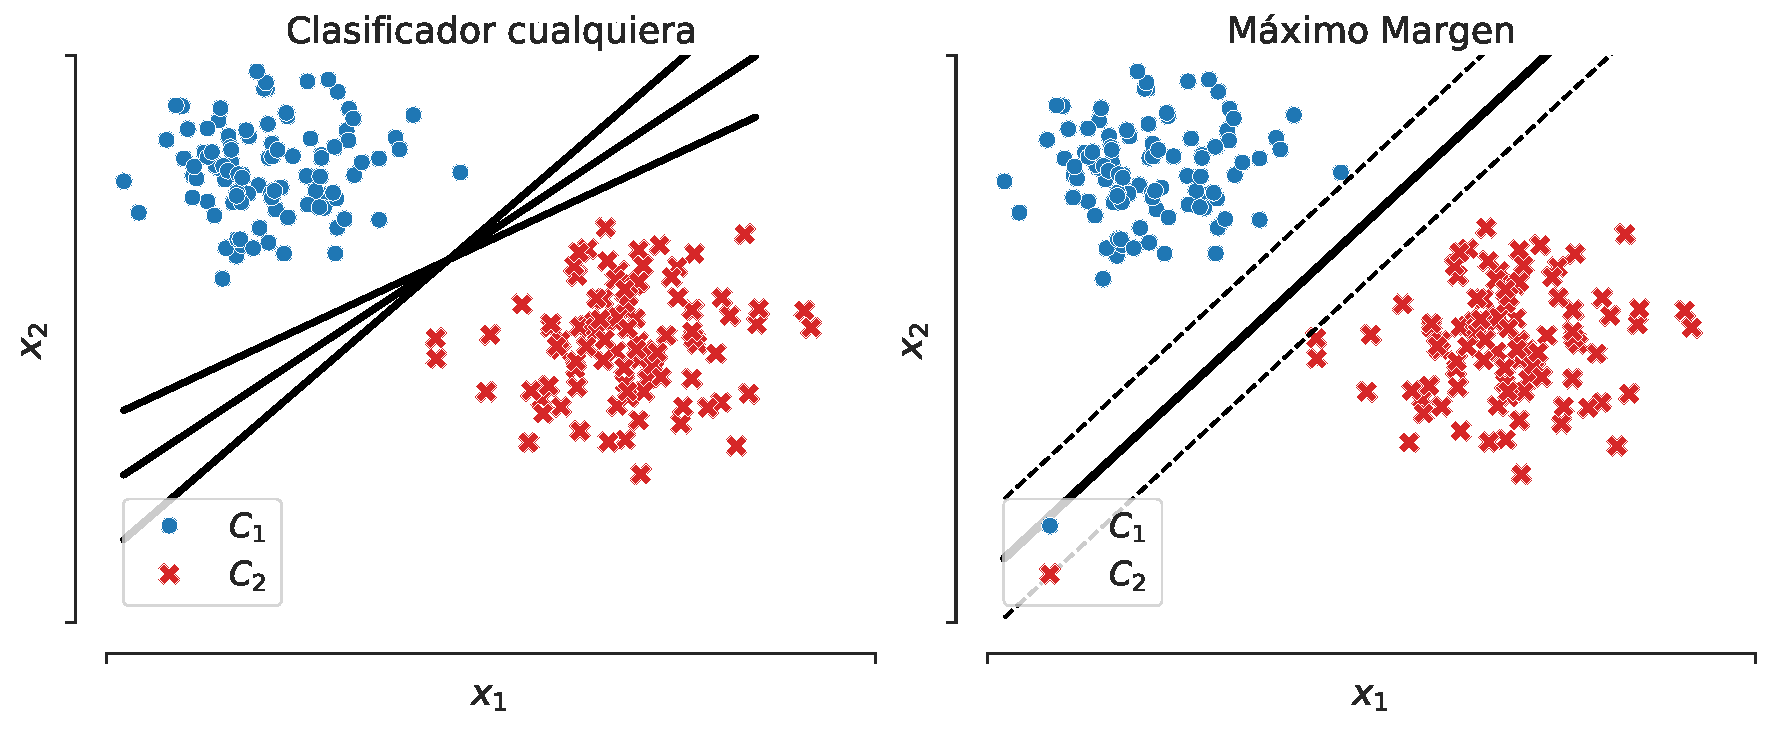
\includegraphics[width=0.9\textwidth]{img/cap5_max_margen.pdf}
    \caption{Clasificadores lineales: varios clasificadores (izquierda) y clasificador de máximo margen (derecha)}
    \label{fig:maxim_marg} 
\end{figure}

Aquí entonces aflora la siguiente pregunta, como todas los clasificadores en la Fig.~\ref{fig:maxim_marg} (izquierda) separan de forma correcta los datos disponibles, ¿cuál de ellos debemos elegir? Elegiremos un \emph{clasificador de máximo margen}, es decir, el clasificador que nos entregue la máxima separación entre los datos y las regiones definidas como correspondiente a cada clase. Una ilustración del clasificador de máximo margen se presenta en la Fig.~\ref{fig:maxim_marg} (derecha). En donde se ve que encontrar este clasificador es equivalente a encontrar una \emph{cinta} de ancho máximo que separe los datos de ambas clases.\\


El argumento de ocupar dicho criterio es la búsqueda de buenas propiedades de generalización. Intuitivamente, esta propiedad se obtiene debido a que asumiendo que los datos generados en cada clase  provienen de una distribución latente, es de esperar que si se obtienen nuevos datos desde la misma distribución, estos estén cerca de los datos observados inicialmente. De este forma, con el máximo margen se pretende maximizar la probabilidad de que los nuevos datos de clase 1 (cf. -1) sean bien clasificados también.\\

Una propiedad clave del clasificador de máximo margen es que este queda definido únicamente por algunos datos, ver Fig.~\ref{fig:maxim_marg} (derecha). Esto inmediatamente resuelve el problema de desbalances de clase o de que las clases tengan formas distintas (problema mencionado en clasificación con mínimos cuadrado o con el discriminante de Fisher). Es decir, la solución de máximo margen se mantiene si agregamos datos (de cualquier clase) que están fuera del margen. Los datos (o vectores, pues recordemos que $x\in\R^M$) que definen el margen los llamaremos vectores de soporte (\emph{support vectors}), cuya función es restringir la rotación y expansión del margen.\\

Finalmente, una diferencia fundamental entre un clasificador que se enfoca en el margen y otros métodos que que hemos visto (e.g., na\"ive Bayes, regresión lineal, regresión logística) es que estos últimos aprenden incorporando todos los datos para formar la respuesta, no solo los que están en el margen. En cambio, SVM define el clasificador utilizando únicamente los vectores soporte ya que si bien todos los datos se debe analizar para encontrar los vectores soporte, los datos que no son vectores soporte no toman parte en la solución final (ni en las predicciones).

\subsection{Formulación del problema}

Denotemos un conjunto de entrenamiento $\{x_i\}_{i=1}^N$, con clases $\{1,-1\}$ linealmente separable y recordemos que un hiperplano de separación está definido mediante
\begin{equation}
    \{x\in \R^n | w^\top x + b = 0 \},\label{ec:hiperplano_svm}
\end{equation}
donde $w\in \R^n$ es el vector perpendicular al hiperplano y $b\in \R$ es el \emph{offset}. De esta forma, si $w^\top x + b >0$ se le asignará a $x$ la clase 1, mientras que si $w^\top x + b <0$ se le asignará a $x$ la clase -1.\\

El problema de clasificación consiste en encontrar dichos parámetros de acuerdo a algún criterio, en este caso es el criterio del máximo margen. Notemos en primer lugar que este problema no tiene solución única, pues si $(w,b)$ son solución entonces $(\lambda w, \lambda b)$, $\lambda>0$ también lo son. Para evitar esta \emph{invarianza} con tal de que el problema tenga solución única, podemos imponer una restricción sobre los bordes del margen. Denotando vectores soporte de cada clase mediante $x_{+}$ y $x_{-}$, se impone que para todo vector soporte $x_+$, $x_-$, estos pertenezcan a su respectiva clase, es decir:
\begin{align}
 	w^\top x_{+} + b &= 1 \label{ec:borde_svm1}\\
 	w^\top x_{-} + b &=  -1\label{ec:borde_svm2}
 \end{align}
 donde estos vectores soportes puede no ser únicos. Observemos que si bien aún no sabemos cuales son los vectores de soporte, podemos imponer esta restricción de todas formas, las que se van a traducir en las restricciones del problema de optimización que definirá la solución del problema de clasificación.\\
 
 Además, es importante ver que las restricciones anteriores implican que $w\neq 0$, lo cual será importante más adelante cuando haya que justificar que el funcional a maximizar es estrictamente cóncavo.

Notemos que las ecs.~\eqref{ec:hiperplano_svm},\eqref{ec:borde_svm1} y \eqref{ec:borde_svm2} definen tres hiperplanos paralelos, pues todos tienen el mismo parámetro $w$. La Fig.~\ref{fig:clasif_margen} ilustra las muestras de cada clase junto con estos tres hiperplanos, donde además se muestra el vector unitario perpendicular a (todos) estos hiperplanos dado por $\frac{w}{||w||}$. El ancho del {margen}, denotado por $m$, es la distancia entre la región de decisión y cualquiera de las clases, y es igual a la mitad de la diferencia entre ambos vectores de soporte, proyectada en la dirección normal del hiperplano, es decir, 
\begin{align}
m &= \frac{1}{2} \norm{\operatorfont{proy}_w(x_+-x_-)} = \frac{1}{2} \norm{x_+-x_-}\cos(\theta) \\
&= \frac{1}{2}\norm{x_+-x_-} \left(\frac{w^\top(x_+-x_-)}{\norm{w}\cdot\norm{x_+-x_-}}\right)\\
& =\frac{1}{2\norm{w}} w^\top(x_+ - x_-)
\end{align}

Donde se usó el hecho de que $\cos\left(\measuredangle(x,y)\right) = \frac{\langle x,y\rangle}{\norm{x}\norm{y}}$.

\begin{figure}[ht]
    \centering
    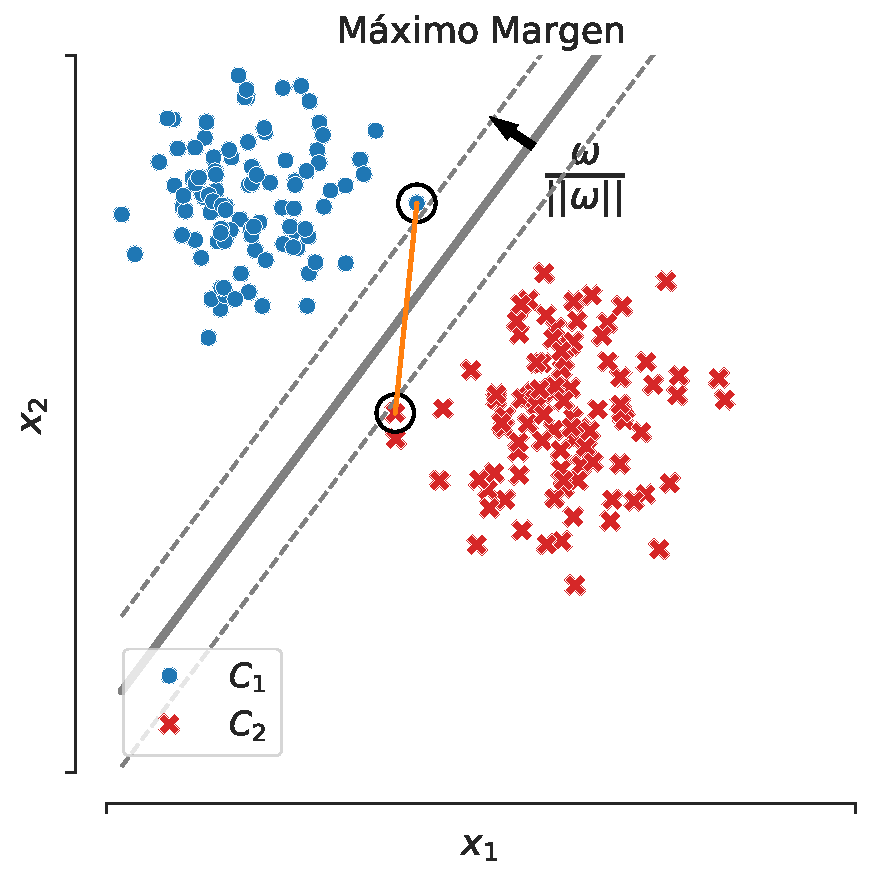
\includegraphics[width=0.4\textwidth]{img/cap5_max_margen2.pdf}
    \caption{Clasificación de máximo margen. Clases denotadas por puntos azules y cruces rojas, región de decisión en gris sólido y bordes del margen en línea punteada. La línea naranja representa la  el vector diferencia $(x_+ - x_{-})$ y la flecha negra el vector unitario $\frac{w}{||w||}$. Los vectores soporte están indicados con un círculo negro.}
    \label{fig:clasif_margen}
\end{figure}

Veamos que el ancho del margen $m$ no depende explícitamente de los vectores soporte al incorporar las restricciones en las ecs.~\eqref{ec:borde_svm1}-\eqref{ec:borde_svm2}:

\begin{align}
    m &= \frac{1}{2||w||} \left( (w^\top x_{+}) - (w^\top x_{-})\right)\nonumber\\
    &= \frac{1}{2||w||} \left((1-b) - (-1-b)\right)\nonumber\\
    &= \frac{1}{||w||}\label{eq:margen}
\end{align}
Además, consideremos la siguiente codificación para las clases:
\begin{alignat}{3}
    y_i&=+1 &&\Leftrightarrow w^\top x_i + b \geq +1 \label{eq:codif_svm1}\\
    y_i &=-1 &&\Leftrightarrow w^\top x_i + b \leq -1\label{eq:codif_svm2}
 \end{alignat}
 
En base a la expresión de la ec.~\eqref{eq:margen} para el ancho del margen y la codificación de clases anterior, podemos formular el problema de clasificación de máximo margen mediante  siguiente problema de optimización:
\begin{equation}
\begin{aligned}
& \underset{w,b}{\text{max}}
& & \frac{1}{||w||}\\
& \text{s.a}
& & y_i (w^\top x_i +b) \geq 1, \; i \in\{ 1, \ldots, N\}
\end{aligned}
\end{equation}
Lo cual simplemente quiere decir que se está maximizando el ancho del margen, sujeto a que todas las muestras estén bien clasificadas. Es importante notar que este problema es factible solo si las clases son linealmente separable ya que restricción exige que todas las muestran queden bien clasificadas.\\

Para evitar problemas de diferenciablidad del recíproco de la raíz cuadrada en el objetivo del problema de optimización anterior, sobretodo cuando $w$ es cercano a 0, consideraremos la siguiente formulación equivalente del problema anterior:
\begin{equation}
\begin{aligned}
(P)\quad & \underset{w,b}{\min}
& & \frac{1}{2}||w||^2\\
& \text{s.a}
& & y_i (w^\top x_i +b) \geq 1, \; i \in\{ 1, \ldots, N\}
\end{aligned}
\end{equation}
Este problema de optimización con restricciones puede ser resuelto mediante el método de Lagrange, donde resolvemos el \emph{problema dual} (ver anexos), el cual tiene una estructura más ``amigable'' para resolver. Además, luego veremos que la resolución mediante este método es fundamental para la extensión no-lineal de SVM.\\

El lagrangiano del problema anterior está dado por:
\begin{equation}
    L(w,b,\alpha) = \frac{1}{2}||w||^2 + \sum\limits_{i=1}^{N} \alpha_i \left(1-y_i (w^\top x_i +b)\right)\label{eq:lagrangiaano_svm}
\end{equation}
donde hemos denotado los multiplicadores de Lagrange mediante $\alpha = (\alpha_1,\ldots,\alpha_N)^\top$. El lagrangiano dual del problema viene dado por $\theta(\alpha) = \inf\limits_{w,b} L(w,b,\alpha)$ y dado que $L$ es convexo, basta aplicar la condición de primer orden:
\begin{align}
	&\frac{\partial L}{\partial w} = w^\top - \sum_{i=1}^N \alpha_i y_i x_i^\top = 0 \implies \overline{w} = \sum_{i=1}^N \alpha_i y_i x_i\\
	&\frac{\partial L}{\partial b} = -\sum_{i=1}^N \alpha_i y_i = 0 \implies \sum_{i=1}^N \alpha_i y_i = 0
\end{align}

Por lo tanto, el lagrangiano dual tiene la siguiente forma:
\begin{align}
	\theta(\alpha) &= L(\overline{w},\overline{b},\alpha) = \frac{1}{2} \left\langle \sum_{i=1}^N \alpha_i y_i x_i,\sum_{j=1}^N \alpha_j y_j x_j \right\rangle + \sum_{i=1}^N \alpha_i - \sum_{i=1}^N \alpha_i y_i \left\langle\sum_{j=1}^N \alpha_j y_j x_j , x_i \right\rangle - b\sum_{i=1}^N \alpha_i y_i  \\
	&= \frac{1}{2} \sum_{i,j=1}^N \alpha_i y_i \alpha_j y_j \langle x_i,x_j\rangle + \sum_{i=1}^N \alpha_i - \sum_{i,j=1}^N \alpha_i y_i \alpha_j y_j \langle x_j,x_i\rangle = \sum_{i=1}^N \alpha_i - \frac{1}{2} \sum_{i,j=1}^N \alpha_i \alpha_j y_i y_j \langle x_i,x_j\rangle
\end{align}

Donde en la penúltima igualdad se usó el hecho de que $\sum\limits_{i=1}^N \alpha_i y_i = 0$ de acuerdo a la segunda CPO sobre $L$.\\

Finalmente, el problema dual consiste en maximizar $\theta(\alpha)$ sujeto a que $\alpha\geq 0$, es decir:


\begin{equation}
\begin{aligned}
(D)\quad & \underset{\alpha}{\max}
& & \sum\limits_{i=1}^{N}\alpha_i - \frac{1}{2} \sum\limits_{i,j=1}^{N} \alpha_i \alpha_j y_i y_j \langle x_i, x_j\rangle\\
& \text{s.a}
& & \sum\limits_{i=1}^{N} \alpha_i y_i= 0 \\
& &  &\alpha_i \geq 0
\end{aligned} \label{eq:dualSVM}
\end{equation}

La primera restricción se heredó de la CPO impuesta sobre $L$ al calcular $\theta(\alpha)$. Este problema es del tipo QP (\emph{quadratic programming}), para el cual existen variados métodos para resolverlo de manera óptima y eficiente. Por otra parte,

\begin{equation}
\sum\limits_{i,j=1}^{N} \alpha_i \alpha_j y_i y_j \langle x_i, x_j\rangle = \sum\limits_{i,j=1}^{N}  \alpha_i \langle   y_i x_i,  y_jx_j\rangle \alpha_j = \alpha^\top \Lambda \alpha,
\end{equation}
 
Donde $\Lambda\in\R^{N\times N}$ corresponde a una matriz de Gram (en alguna base) por lo que es definida positiva ya que para $\alpha\neq 0$:

\begin{equation}
	\alpha^\top \Lambda \alpha = \sum\limits_{i,j=1}^{N}   \langle   \alpha_i y_i x_i,  \alpha_j y_jx_j\rangle = \left\langle\sum\limits_{i=1}^{N}      \alpha_i y_i x_i,  \sum\limits_{j=1} \alpha_j y_jx_j\right\rangle = \norm{\sum\limits_{i=1} \alpha_i y_i x_i}^2 = \norm{\overline{w}}^2>0 
\end{equation}

Además, se tiene la siguiente propiedad:

\begin{lemma}
	$A$ es definida positiva si y solo si $f(x)= x^\top Ax + b^\top x + c$ es estrictamente convexa.
\end{lemma}

\begin{proof}
	Basta verlo para la forma cuadrática $f(x)=x^\top Ax$. Sea $\lambda\in (0,1)$ y $x,y\in\R^n$ con $x\neq y$, entonces:
\begin{align*}
	&\left(\lambda x+(1-\lambda)y\right)^\top A \left(\lambda x+(1-\lambda)y\right) <\lambda x^\top Ax + (1-\lambda)y^\top Ay\\
			\iff &\lambda^2 x^\top Ax + (1-\lambda)^2 y^\top Ay + \lambda(1-\lambda)x^\top Ay + \lambda(1-\lambda)y^\top Ax < \lambda x^\top Ax+(1-\lambda)y^\top Ay\\
			\iff & \lambda(1-\lambda)x^\top Ax+\lambda(1-\lambda)y^\top Ay-\lambda(1-\lambda)y^\top Ay> 0\\
			\iff & x^\top Ax+y^\top Ay-x^\top Ay-y^\top Ax> 0\\
			\iff & (x-y)^\top A(x-y)> 0, \forall x,y\in \R^n:x\neq y\\
			\iff &A \text{ es definida positiva}
\end{align*}
\end{proof}

Luego, el funcional de SVM es estríctamente cóncavo, lo cual implica que el máximo del problema es único.\\

 Una vez resuelta la formulación dual (i.e., se han encontrado los valores óptimos para $\alpha$), la predicción de un nuevo punto $x_\star$ es de la forma 
\begin{equation}
 	\hat{y}(x_\star)= \text{sgn} (\overline{w}^\top x_\star + b) = \text{sgn}\left(\left[\sum\limits_{i=1}^{N} \alpha_i y_i \langle x_i, x_\star\rangle\right] + b\right)
 \end{equation}
 
Finalmente, por el teorema de holgura complementaria, para $\alpha$ óptimo se tiene que
\begin{equation}
	\alpha_i \left(1-y_i (\overline{w}^\top x_i +b)\right) = 0,\quad \forall i\in\{1,\ldots,N\}\implies \alpha_i=0\text{ para todo $x_i$ fuera del margen.}
\end{equation}

y consecuentemente, $x_i$ no aporta en la predicción $\hat{y}$. Esta propiedad es la que mencionábamos al principio: la predicción de clase solo depende de los vectores soporte, i.e., los que están en el margen. Esto ayuda a resolver el problema de optimización de manera más rápida, ya que en realidad solo algunas variables duales $\alpha_i$ serán no nulas (las correspondiente a los vectores que están en el borde del margen). Normalmente se ocupan heurísticas para encontrar y descartar rápidamente que vectores no son de soporte y así resolver un problema mas simple (ver, por ejemplo, el método de \emph{Sequential Minimal Optimization}). 


\begin{remark} Notemos que las características $\{x_i\}$ solo aparecen en forma de productos internos entre ellas mismas en la solución del método SVM, lo cual se puede ver desde la formulación de problema de optimización dual en la ec.~\eqref{eq:dualSVM}. Esto es clave para la extensión no lineal de SVM, pues no necesitamos operar directamente  con los valores de las entradas o características, sino con los productos punto entre ellas. En particular, si tenemos $N$ entradas de $M$ dimensiones, solo necesitamos los $N(N+1)/2$ productos puntos entre ellos y no todos los $NM$ valores, lo cual es particularmente relevante en caso que $M$ sea muy grande o incluso cuando $M=\infty$ (e.g., cuando las características $\phi:x_i\mapsto \phi(x)$ son funciones).
\end{remark} 

\subsection{Margen suave}

El planteamiento anterior tiene dos debilidades: la primera es que nuestros datos no siempre serán separables, y la segunda es que, incluso si los datos son linealmente separables, nuestro clasificador puede ser muy sensible a nuevos datos. Esto es ilustrado en la Fig.~\ref{fig:svm_softmargin}, donde el clasificador de máximo margen sin \emph{outlier} (izquierda) es muy distinto, o no-robusto, al obtenido en el caso de un \emph{outlier} (encerrado en púrpura). En general, queremos que nuestro estimador sea robusto a este tipo de datos, tal como lo es la regresión lineal frente a observaciones ruidosas. 

\begin{figure}[ht]
    \centering
    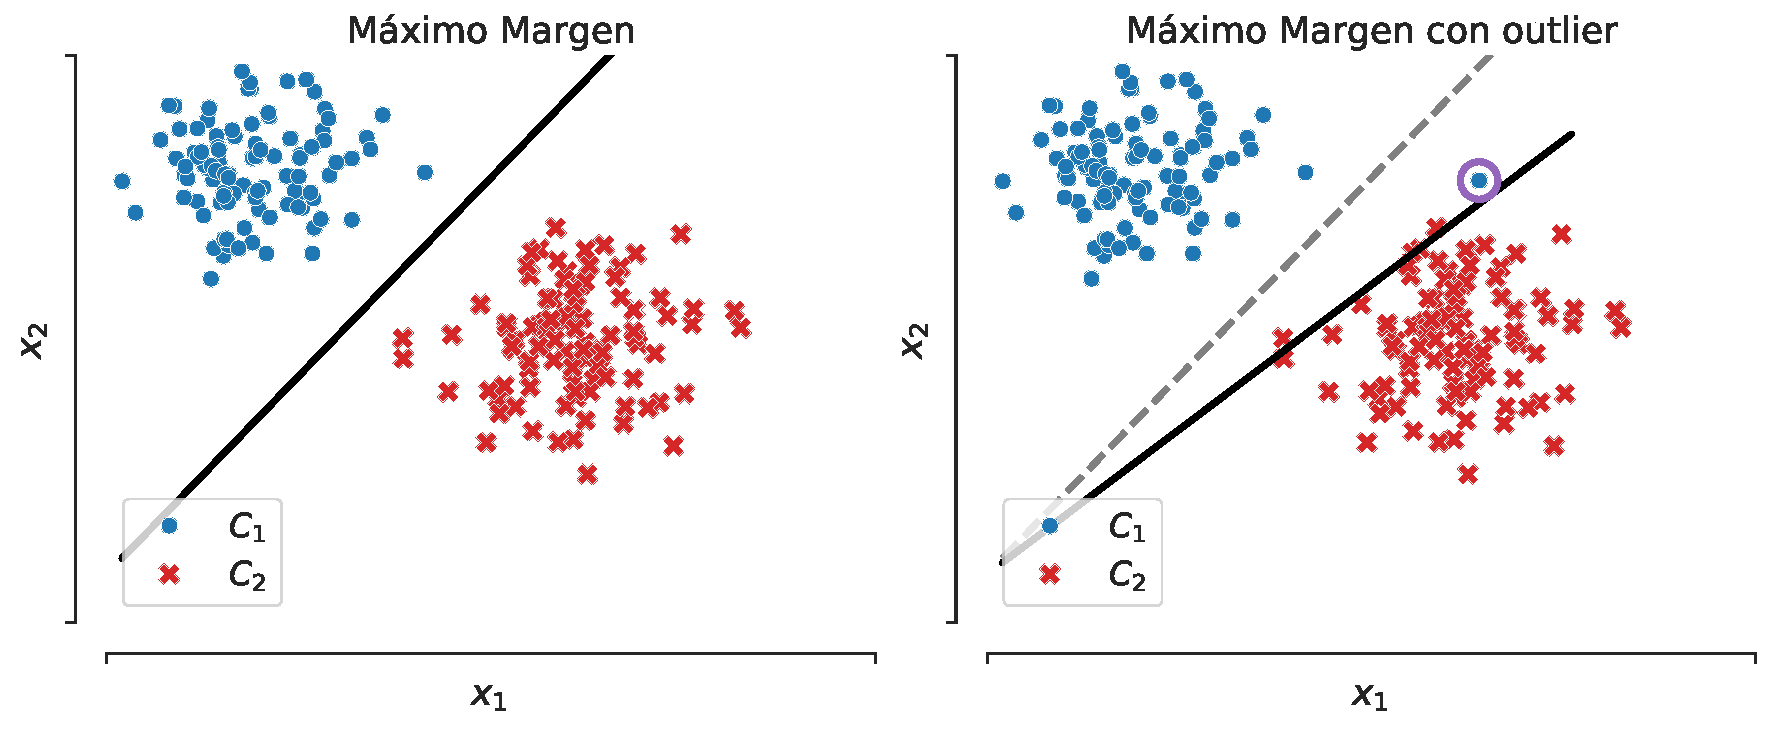
\includegraphics[width=0.9\textwidth]{img/cap5_margen_suave}
    \caption{Sensibilidad del máximo margen al agregar un nuevo dato: a la izquierda el caso sin \emph{outlier} y a la derecha el caso con \emph{outlier}, donde la solución anterior se muestra con la línea punteada.}
    \label{fig:svm_softmargin}
\end{figure}

Para considerar datos que son no posibles de clasificar con el clasificador lineal de máximo margen, podemos introducir las llamadas ``variables de holgura'' (\emph{slack variables}). Estas tienen el objetivo de permitir al clasificador admitir algunos datos incorrectamente clasificados, aún maximizando el margen. Específicamente, esto se logra reemplazando las restricciones para los datos mal clasificados (considerados \emph{outliers}) directamente en la formulación del problema de optimización, de esta forma, la \textit{mayoría} de los datos se clasifican de forma correcta con la finalidad de tener un modelo robusto.

\newpage

La formulación del problema de clasificación que \emph{perdona} algunos datos mal clasificados mediante la utilización de variables de holgura $\{\xi_i\}_{i=1}^N$ es la siguiente:

\begin{equation}
\begin{aligned}
(P)\quad & \underset{w,b, \xi}{\text{min}}
& & \frac{1}{2}||w||^2 + c\sum\limits_{i=1}^{N} \xi_i \\
& \text{s.a}
& & y_i (w\cdot x_i +b) \geq 1 - \xi_i,\;\xi_i\geq0,\; i \in\{ 1, \ldots, N\}
\end{aligned}
\end{equation}
donde $c>0$ es un hiperparámetro. Observemos que la introducción del término $c\sum_{i=1}^{N} \xi_i$ en la función de costo puede ser interpretada como una regularización, tal como lo hicimos con mínimos cuadrados. En efecto, de las restricciones del problema anterior, podemos ver que los $\xi$ indican qué tan mal clasificado está un punto, donde: 
\begin{itemize}
    \item si $\xi_i = 0$, entonces el dato $x_i$ está al lado correcto del plano y obtenemos el problema anterior
    \item si $0<\xi_i <1$, entonces $x_i$ está al lado correcto del plano, pero está dentro del margen, 
    \item si $\xi_i>1$, entonces el punto esta al lado incorrecto del plano.
\end{itemize}
Estas tres condiciones son ilustradas en la Fig.~\ref{fig:soft_margin}.
\begin{figure}[ht]
    \centering
    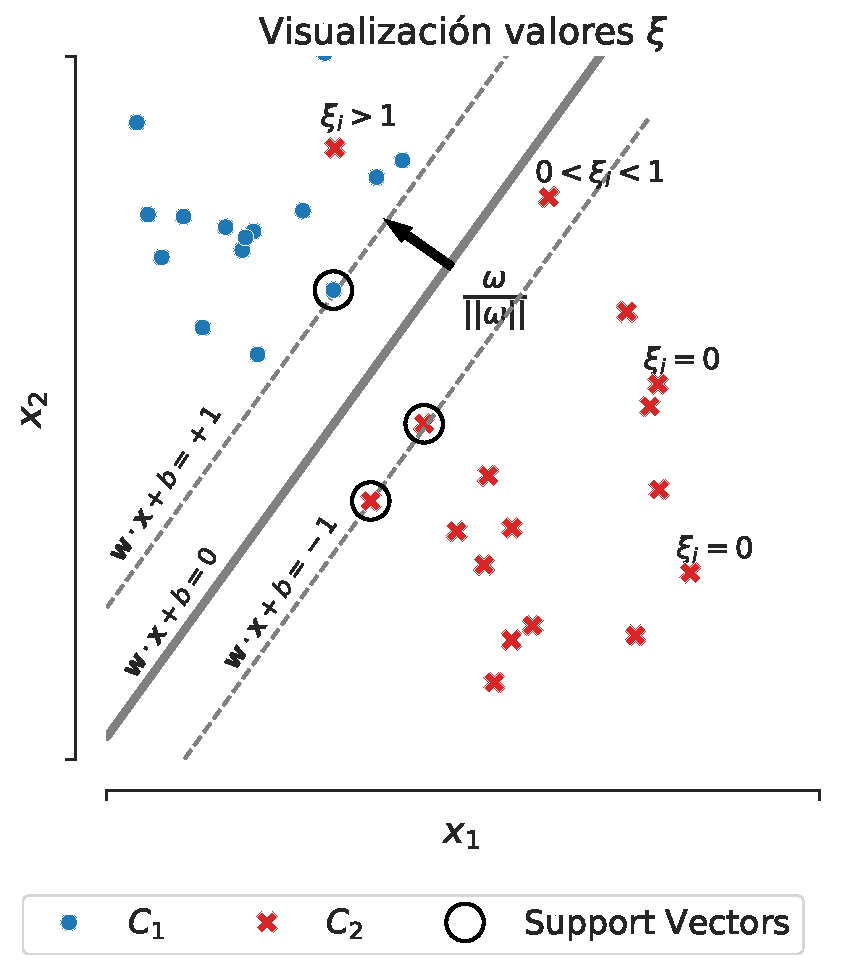
\includegraphics[width=0.45\textwidth]{img/cap5_max_margen3}
    \caption{Valores para las variables de holgura $\xi$ en distintas regiones del espacio de entrada.}
    \label{fig:soft_margin}
\end{figure}

Procediendo de la misma forma que en el caso anterior, el dual de este problema es:
\begin{equation}
\begin{aligned}
(D)\quad & \underset{\alpha}{\text{max}}
& & \sum\limits_{i=1}^{N}\alpha_i - \frac{1}{2} \sum\limits_{i,j=1}^{N} \alpha_i \alpha_j y_i y_j \langle x_i, x_j\rangle\\
& \text{s.a}
& & \sum\limits_{i=1}^{N} \alpha_i y_i= 0 \\
& &  &0 \leq \alpha_i \leq c
\end{aligned}
\end{equation}
Esta solución similar al caso anterior y también se puede resolver con técnicas de programación cuadrática, en particular, su solución también existe y es única. La diferencia entre ambas soluciones (con y sin variables de holgura) está dada por el hecho de que los multiplicadores de Lagrange ahora están acotados por el hiperparámetro $c$, el que representa la importancia que se da a la suma de las variables de holgura versus el ancho del margen en la función de costo del problema de optimización.\\

Por último, ¿cómo definir el parámetro $c$? Es posible responder esta pregunta en relación al \textit{bias-variance tradeoff}. Notemos que $\xi_i>1$ si la muestra $x_i$ está mal clasificada, entonces el término $\sum_{i=1}^{N} \xi_i$ es una cota superior para la cantidad de muestras mál clasificadas. Consecuentemente, el hiperparámetro $c$ es un coeficiente (\emph{inverso}) de regularización, pues su magnitud controla el balance entre la maximización del margen y la cantidad muestras mal clasificadas. En particular, para un $c$ muy alto la cantidad de muestras mal clasificadas tiene mucho peso relativo comparada contra el ancho del margen en el funcional de minimización, con lo que la solución óptima tendrá un margen muy angosto y pocas (si es que hay alguna) muestras mal clasificadas. En efecto, si $c\to\infty$, se recupera la formulación del \emph{margen duro} y su misma solución de máximo margen (en el caso de que el problema sea efectivamente linealmente separable), pues solo se podrá resolver el problema si todas las variables de holgura son nulas. Por el contrario, para un $c$ pequeño el margen tiene más importancia que la cantidad de datos incorrectamente clasificados, con lo que se encontrará un margen amplio con varias muestras mal clasificadas. Es de esperar que un $c$ pequeño (margen amplio) tenga mejor capacidad de generalizar a nuevos datos con menor varianza, mientras que un $c$ grande puede sobreajustar a los datos disponibles, reportando peor desempeño \emph{out-of-sample}. Por esto hemos dicho que $c$ es análogo a un coeficiente \emph{inverso} de regularización, pues mientras más pequeño, más regular es la solución. \\

Al no conocer los estadísticos de los datos, en la práctica ajustamos el hiperparámetro $c$ mediante validación cruzada.

\subsection{Método de kernel}

El clasificador SVM (tanto con margen duro o blando) tiene una propiedad muy beneficiosa en el caso linealmente separable: la solución siempre existe, es única y se puede encontrar. Sin embargo, no tenemos ninguna garantía en los casos no separables, los cuales afloran usualmente en la práctica. Consideremos el problema de clasificar una base de datos generadas con una función ``o exclusivo'', o ``XOR'', presentada en la Figura~\ref{fig:xor}. Estos datos no son linealmente separables, con lo que al calcular el clasificador óptimo  de SVM no llegaríamos a ninguna solución coherente ya que el problema es infactible, sin embargo, notemos que es posible diseñar una característica particular para este conjunto donde sí son separables. 

\begin{figure}[ht]
    \centering
    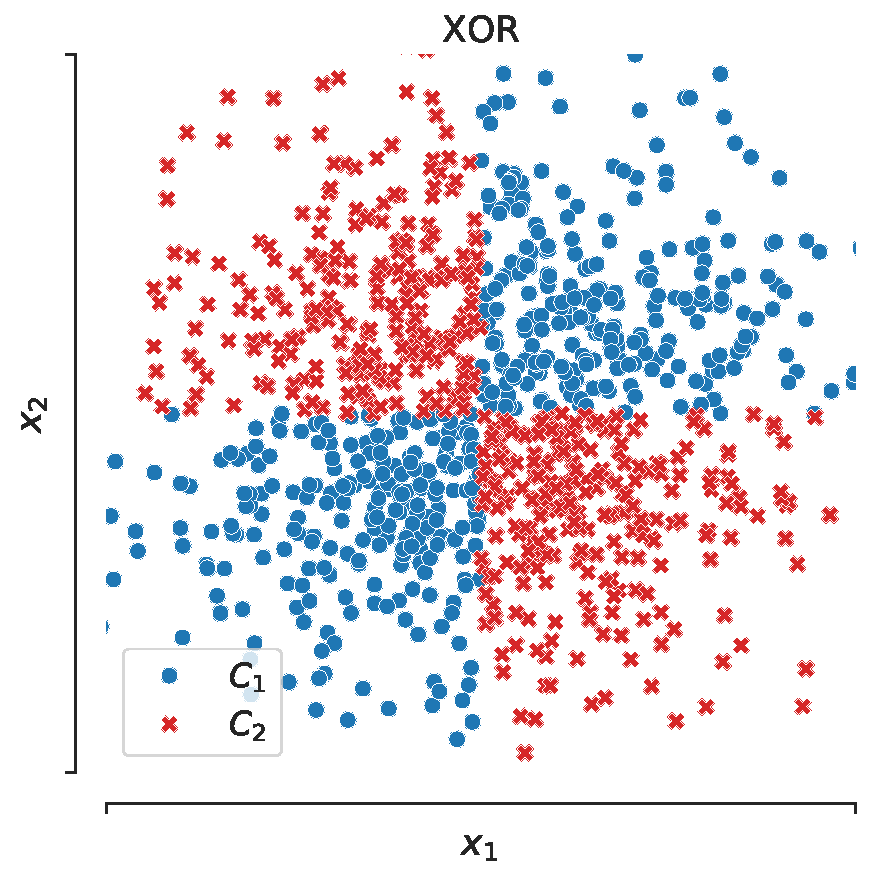
\includegraphics[width=0.35\textwidth]{img/cap5_xor}
    \caption{Datos XOR: no son linealmente separables.}
    \label{fig:xor}
\end{figure}

En efecto, consideremos el mapa desde  $\R^2$ a $\R^3$ definido mediante
\begin{equation}
    \phi: [x_1, x_2]^\top \mapsto [x_1, x_2, x_1 x_2]^\top
\end{equation}
y observemos que este permite clasificar de forma lineal (y trivial) las clases del problema XOR: ambas quedan clasificadas mediante el plano $z=0$ en $\R^3$, esto es ilustrado en la Fig.~\ref{fig:xor_proyectado}. La función $\phi$ es un ejemplo de una ingeniería de características como las vistas en el capítulo de regresión no lineal, en este caso particular, la característica relevante era precisamente $x_1x_2$.

\begin{figure}[ht]
    \centering
    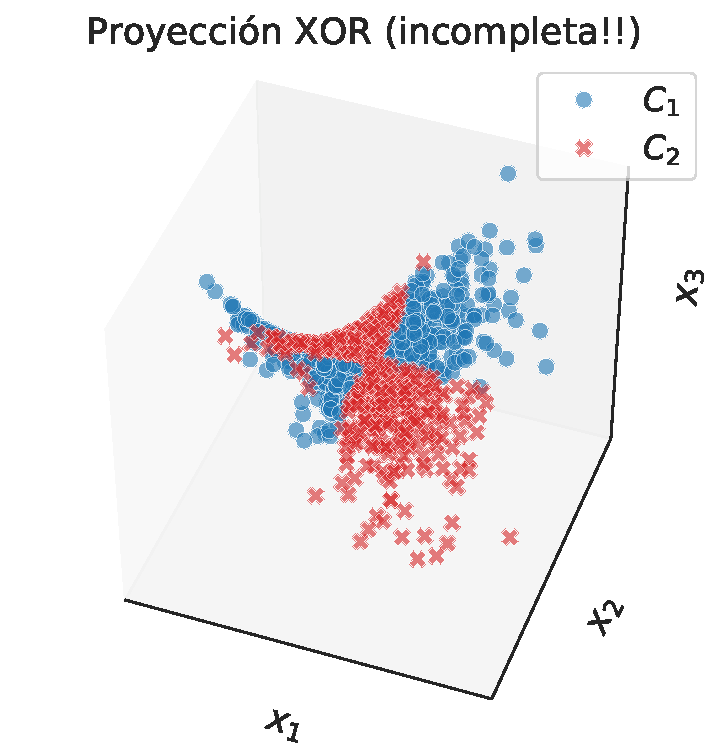
\includegraphics[width=0.45\textwidth]{img/cap5_xor_3d_proyeccion}
    \caption{Los puntos rojos y azules corresponden a los datos mapeados a través de $\phi$. El plano $z=0$ es capaz de separar puntos rojos y puntos azules en este nuevo espacio.}
    \label{fig:xor_proyectado}
\end{figure}

%%VOLVER A PROYECTAR

\begin{remark}
En el caso del problema XOR conocíamos la característica apropiada, sin embargo, en el caso general no es claro cuál debe ser ``el buen $\phi$''. A pesar de esto, notemos que tanto para la formulación con margen duro o blando de SVM, la solución solo requerirá que seamos capaces de calcular los productos internos entre las características de cada entrada. Es decir, si consideramos un $\phi$ arbitrario para nuestro problema de clasificación, solo necesitaríamos calcular los productos puntos de la forma
\begin{equation}
    \langle \phi(x_i) , \phi(x_j) \rangle 
\end{equation}
para todo $x_i,x_j$ en el conjunto de entrenamiento. 
\end{remark}

Podemos entonces aplicar la siguiente intuición: seguramente no podemos encontrar el $\phi$ exclusivo de cada problema, sino que podemos utilizar uno (o una clase) que sea muy general, complejo, o ``universal''. Esperamos que esta característica general nos sirva para una gran cantidad de problemas, donde tenemos la garantía de que lo podremos usar como parte de SVM si somos capaces de calcular su producto interno. Además, por ``general'' podemos entender ``de alta dimensión'': podríamos pensar que para un problema en el cual no sabemos el buen $\phi$, podemos considerar incorporar e incorporar características, con lo cual tendríamos una ``característica agregada'' de alta dimensión, esperando que alguno de los términos agregados sea el que efectivamente separa las clases. Si bien no está garantizada la separabilidad lineal al combinar características, al agregar dimensiones los datos están cada vez más separados debido a la maldición de la dimensionalidad y se puede probar que en dimensión infinita, siempre se podrá separar linealmente.

\begin{figure}[h]
    \centering
    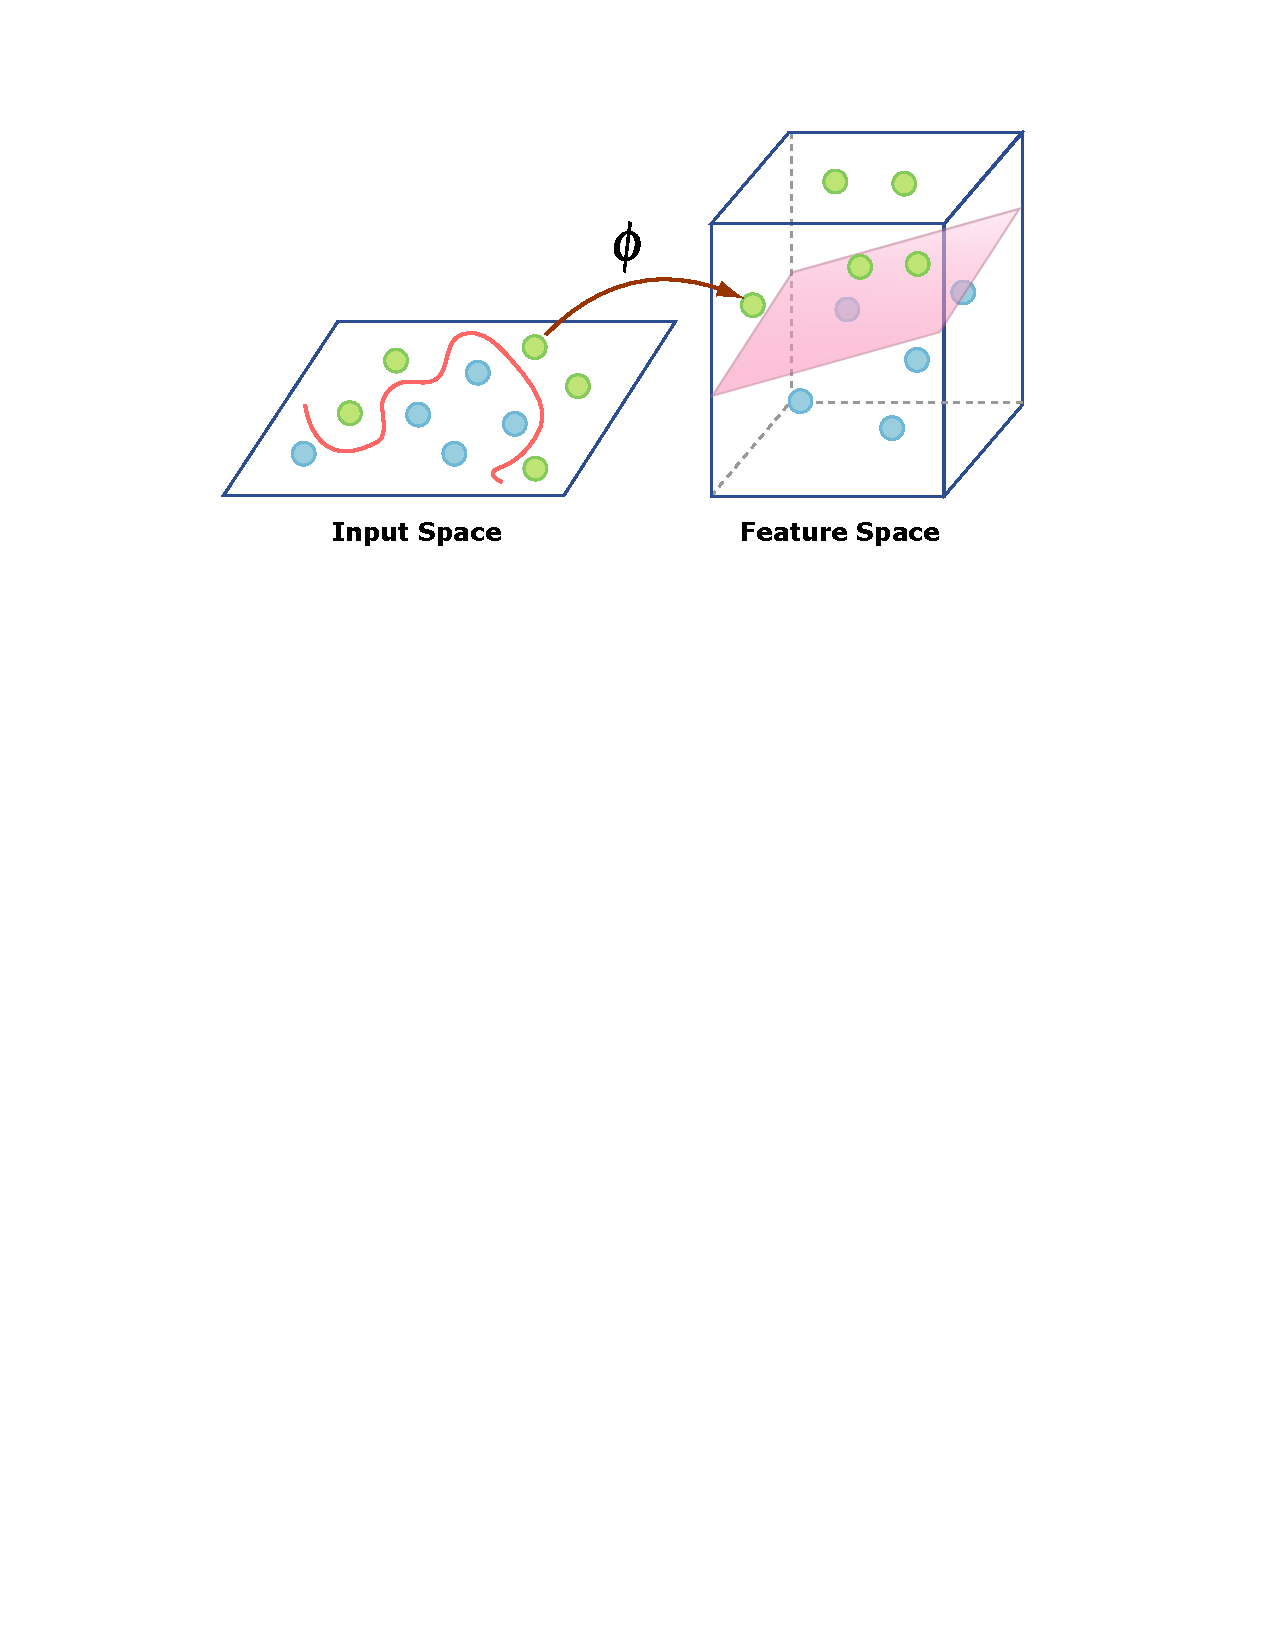
\includegraphics[width=0.45\textwidth]{img/cap5_kernelSVM}
    \caption{Separación lineal en un espacio de dimensión mayor. Imagen obtenida de MIT OpenCourseWare (MIT 15.097 course).}
\end{figure}



\newpage

Para encontrar estos $\phi$ generales, veamos la siguiente definición
\begin{definition}[Mercer kernel]
    Un Mercer kernel es una función continua $K: X\times X \to \R$ tal que
\begin{itemize}
    \item Es simétrica $K(x_1 , x_2 ) = K (x_2 , x_1)$
    \item Es definida positiva, es decir
    $$\int_{X^2} K(x_1, x_2)g(x_1) g(x_2) dx_1 dx_2\geq 0,$$
    para toda función $g:X\rightarrow\R$ continua. El nombre de de esta propiedad derivada de su similitud con las matrices definidas positivas: si $g$ se mira como vector de $\R^X$, entonces la expresión anterior representa a $g^\top Kg\leq 0$.
\end{itemize}

\end{definition}

De esta forma, se tiene el siguiente teorema de analisis funcional que sustenta la utilización de kernels en los algoritmos de aprendizaje automático:


\begin{theorem}[teorema de Mercer (simplificado)]
	Sea $K: X\times X \to \R$ un Mercer kernel, entonces existe un espacio de Hilbert $\left(\mathcal{H},\langle,\rangle\right)$ y una función $\phi: X \to \mathcal{H}$ tal que:
	\begin{equation}
    K(x_1, x_2) = \langle \phi(x_1) , \phi(x_2) \rangle
\end{equation}
\end{theorem}

Es decir, existe un mapa de características $\phi$ tal que $K(x_1, x_2)$ representa el producto interno (en algún espacio) de las características de $x_1$ y $x_2$. Además, dicho espacio no es necesariamente de dimensión finita.

\begin{remark}[truco del kernel]
La introducción del concepto de kernel es fundamental en SVM. La definición y el teorema anterior nos dicen que para cualquier función simétrica y definida positiva $K$, existe una función $\phi$, que puede ser incluso de dimensión infinita, tal que la evaluación del kernel en dos puntos cualquiera equivale al producto interno entre dos evaluaciones de $\phi$ en los mismos puntos, es decir, $K(x_1,x_2)$ representa un producto interno en algún espacio de características. Esto, sumado al hecho de que la solución de SVM solo requiere del cálculo de productos internos, nos permite construir \emph{kernel SVMs}, donde parametrizamos directamente el producto interno en el problema de optimización mediante el kernel, pues esto da la garantía que el mapa de características $\phi$ existe. El caso interesante es cuando ocupamos un kernel que corresponde a un $\phi$ infinito dimensional, pues estamos efectivamente realizando la clasificación en un espacio de dimensión infinita pero con un procedimiento que solo requiere de una cantidad finita de cálculos, esto se llama \emph{el truco del kernel}. Este truco puede aplicarse a cualquier algoritmo en donde las entradas solo aparezcan en la forma de productos punto, proceso que recibe el nombre de \emph{kernelización}. 
\end{remark}

\newpage

 Veamos distintos tipos de kernels y sus propiedades.

\begin{itemize}
    \item   \textbf{Kernel polinomial:}
    \begin{equation}
       K_{pol} (x, y) = (c + x^\top y)^d
    \end{equation}
    donde $c\geq 0$ es un parámetro libre y $d\in\N$ es el orden del polinomio. Para probar que dicha función es un kernel, basta reagrupar los términos buscando formar un producto interno. Para $x,y\in\R^m$, $d=2$ se tiene que: 
    \begin{align}
        K_{pol} (x, y)  &= \left(c + \sum_{i=1}^m x_iy_i\right)^2\\
                        &= \sum_{i=1}^m (x_i^2)(y_i^2) + \sum_{i=2}^m \sum_{j=1}^{i-1} (\sqrt{2}x_ix_j)(\sqrt{2}y_iy_j) + \sum_{i=1}^m (\sqrt{2c}x_i)(\sqrt{2c}y_i) + c^2\\
                        &=\langle \phi_{pol}(x) , \phi_{pol}(y) \rangle
    \end{align}
    donde 
    \begin{equation}
        \phi_{pol}(x) = [x_1^2,\ldots,x_m^2,\sqrt{2}x_1x_2,\ldots, \sqrt{2}x_{m}x_{m-1},\sqrt{2c}x_1,\ldots,\sqrt{2c}x_m,c].
    \end{equation}
    Es decir, al usar el kernel poliomial estamos implícitamente usando un mapa de características que contiene todos los monomios de grado hasta $d=2$ (si $c>0$) o bien todos los monomios de grado igual a $d=2$ (en caso que $c=0$). Más allá de esta ilustración, esto se cumple para cualquier $d\in\N$.
    \item \textbf{Función de base radial (RBF kernel)\footnote{también conocido como kernel exponencial cuadrático o gaussiano.}:} Este kernel está definido por
    \begin{equation}
        K_{RBF} (x , y ) = \sigma^2 \exp\left(-\frac{\norm{x -y}^2}{2l^2}\right).
    \end{equation}
    El mapa de características que induce es de dimensión infinita y las fronteras que entrega son suaves (infinitamente diferenciables). Los hiperparámetros del kernel son $\sigma^2$ (controla la distancia promedio de la función con su media) y $l$ (controla la oscilación de la curva).
        
    \item \textbf{Kernel periódico:}
    \begin{equation}
       K_{per} (x , y) = \sigma^2 \exp\left(- \frac{2\sen^2 \left(\frac{\pi|x -y|}{p}\right)}{l^2}\right).
    \end{equation}
    
    Este kernel es capaz de rescatar características periódicas en los datos (controlados por el parámetro $p$). Los otros parámetros cumplen la misma función que el kernel anterior. 
    
\end{itemize}

Por último, el conjunto de kernels es cerrado bajo sumas y multiplicaciones, lu cual permite construir kernels más complejos combinando otros más simples. Esto será de gran utilidad en procesos gaussianos.

\subsubsection{Kernel ridge regression}

Veamos que es directo kernelizar el método de mínimos cuadrados regularizados visto en la Sección \ref{sub:min_cuad_reg}. En particular, consideremos el caso de regularización cuadrática, el cual, vimos que tiene solución
\begin{equation}
    \theta_{MCR} = \left(\tX^\top\tX +\rho \eye\right)^{-1} \tX^\top Y
    \label{eq:RR_soln1}
\end{equation}
 y consecuentemente, reporta una predicción en base a un nuevo input $x_\star$ dada por $\hat{y}_\star = \theta_{MCR}^\top x_\star$. Como podemos ver, la interacción de las entradas $(\tx_i)_{i=1}^N$ no aparece en la forma de productos internos (lo cual es necesario para la kernelización) ya que $(\tX^\top\tX)_{ij}=\langle\tX^\top_{i\cdot},\tX_{\cdot j}\rangle=\langle\tX_{\cdot i},\tX_{\cdot j}\rangle$, es decir, es el producto interno de las columnas de $\tX$ y no de los datos (recordar que $\tx_i = \tX_{i\cdot}$). Sin embargo, se tiene la siguiente propiedad de inversión:

\begin{lemma} La solución de mínimos cuadrados es equivalente a

\begin{equation}
	\theta_{MCR} = \tX^\top\left(\tX\tX^\top + \rho\eye\right)^{-1}Y
	\label{eq:RR_soln2}
\end{equation}

\end{lemma}

\begin{proof}
	Usando la fórmula de Woodburry (ver anexos)
	
	\begin{equation}
		(A+UCV)^{-1} = A^{-1} - A^{-1}U(C^{-1}+VA^{-1}U)^{-1}VA^{-1}
	\end{equation}
	
considerando $A=\rho\eye$, $U=\tX^\top$, $C=\eye$ y $V=\tX$, se tiene que:
\begin{align}
	\theta_{MCR} &= \left(\frac{1}{\rho}\eye- \frac{1}{\rho}\tX^\top\left(\eye+\frac{1}{\rho}\tX\tX^\top\right)^{-1}\frac{\tX}{\rho}\right)\tX^\top Y=\frac{1}{\rho}\tX^\top \left(\eye- \left(\eye+\frac{1}{\rho}\tX\tX^\top\right)^{-1}\frac{\tX\tX^\top}{\rho}\right)Y\\
	&= \frac{1}{\rho}\tX^\top \left(\eye- \left(\eye+\frac{1}{\rho}\tX\tX^\top\right)^{-1}\left(\eye+\frac{1}{\rho}\tX\tX^\top\right) + \left(\eye+\frac{1}{\rho}\tX\tX^\top\right)^{-1}\right)Y\\
	&= \frac{1}{p}\tX^\top\left(\eye+\frac{\tX\tX^\top}{\rho}\right)^{-1}Y= \tX^\top\left(\tX\tX^\top + \rho\eye\right)^{-1}Y
\end{align}
\end{proof}

Donde ahora $\tX\tX^\top$ sí corresponde a un producto externo de las entradas:

\begin{equation}
	(\tX\tX^\top)_{ij}=\langle\tX_{i\cdot},\tX^\top_{\cdot j}\rangle=\langle\tX_{i\cdot},\tX_{j\cdot}\rangle = \langle \tx_i,\tx_j\rangle
\end{equation}

Además,

\begin{equation}
	\hat{y}_\star = \theta_{MCR}^\top x_\star = Y^\top \left(\tX\tX^\top + \rho\eye\right)^{-1}\tX \tx_\star
\end{equation}

donde $(\tX x_\star)_i = \langle \tilde{x}_i,x_\star\rangle$, lo cual muestra que las entradas solo aparecen en la predicción en forma de productos internos.

\begin{remark}[Costo computacional: dimensión v/s cantidad de datos]
Como $\tX\in\R^{N\times M}$, donde $N$ es la cantidad de datos y $M$ es la dimensión de los datos de entrada, entonces la matriz a invertir en la ec.~\eqref{eq:RR_soln1} es de tamaño $M\times M$, mientras que la matriz a invertir en la ec.~\eqref{eq:RR_soln2} es de tamaño $N\times N$. Como el costo de invertir una matriz es de orden cúbico (dependiendo del método) en su dimensión, será preferible utilizar una de las dos formulaciones en base a qué es mayor, la dimensión o el número de datos. 
\end{remark}

Por otro lado, sea $\phi$ un mapa de características (i.e., una función que recupera las características de una entrada $x$), denotando las características por $\phi_i=\phi(x_i)$ y $\phi_\star = \phi(x_\star)$, se puede hacer la regresión sobre las características:

\begin{equation}
	\Theta=\left(\begin{matrix}
		\phi_1^\top\\
		\vdots\\
		\phi_N^\top
	\end{matrix}\right) \implies \hat{y}_\star = Y^\top \left(\Theta\Theta^\top + \rho\eye\right)^{-1}\Theta \phi_\star
\end{equation}

Luego, si $K$ es un kernel asociado al mapa de características $\phi$, es decir $K(x_i,x_j)=\langle\phi(x_i),\phi(x_j)\rangle$, se tiene que


\begin{equation}
    \hat{y}_\star = Y^\top \left(\Theta\Theta^\top + \rho\eye\right)^{-1}\Theta \phi_\star  = Y^\top \left(K(\tX,\tX) + \rho\eye\right) ^{-1} K(\tX, x_\star),    
\end{equation}

donde se ha hecho abuso de notación al usar argumentos matriciales en el kernel:
\begin{equation}
	K(\tX,\tX)_{ij} = (\Theta\Theta^\top)_{ij} = \langle\phi_i,\phi_j\rangle = K(x_i,x_j)\qquad K(\tX,x_\star)_i = (\Theta\phi_\star)_i = \langle\phi_i,\phi_\star\rangle = K(x_i,x_\star)
\end{equation}

Alternativamente, esta predicción puede ser reordenada para dar 
\begin{equation}
   \hat{y}_\star    = \sum_{i=1}^N h_i K(x_i,x_\star)\label{eq:RR_pred2},
\end{equation}
donde hemos denotado el vector $h\in\R^N$ de la forma $h_i = \left(Y^\top \left(K(\tX,\tX) + \rho\eye\right) ^{-1}\right)_i$. Hay varias observaciones relevantes que podemos hacer con respecto al resultado anterior. 

\begin{remark}[Infinitas características]
Como hemos descrito la predicción de MCR en forma de productos internos, podemos reemplazar las entradas $x$ en las descripción anterior por una característica $\phi(x)$, de dimensión $D$. Luego, si el kernel $K$ tiene asociado un mapa de dimensión infinita, la regresión se hará sobre dicho mapa, buscando separar la entrada en un espacio de dimensión infinita. 
\end{remark}


\begin{remark}[Kernel como similitud]
    Notemos de la expresión anterior que si el kernel $K(x,x')$ es una medida de similitud entre $x$ y $x'$, entonces la predicción de $y_\star$ es una combinación lineal de $h_i$, donde los ponderadores de cada $h_i$ son mayores para los datos $x_i$ que se parecen (con respecto a $K$) a la nueva entrada $x_\star$. A su vez, los valores $h_i$ son una transformación lineal de las entradas $Y$, con lo que la predicción de \emph{kernel ridge regression} combina linealmente salidas conocidas en base a cuán similar a los datos históricos es una nueva entrada. 
\end{remark}

\begin{remark}[Modelo no paramétrico] Como vimos anteriormente, el hecho de que la predicción en la ec.~\eqref{eq:RR_pred2} solo dependa del kernel permite evitar definir explícitamente el mapa de características $\phi$, sino que solo necesitamos el kernel $K$. Esto permite utilizar un kernel (e.g., exponencial cuadrático) que corresponde a un $\phi$ de dimensión infinita, lo que resulta en el parámetro $\theta$ siendo también de dimensión infinita. A pesar de la característica \emph{infinita} de este método, solo necesitamos hacer un cálculo finito para representar $\hat{y}_\star$, esto se puede interpretar como la extracción de la información suministrada por los datos que tenemos $\datos = \{x_1,\ldots,x_n\}$, los cuales son finitos a pesar de que el modelo tenga una ``capacidad'' infinita (ver el Teorema del representante). Una consecuencia de esto es que la predicción en la ec.~\eqref{eq:RR_pred2} depende de todos los elementos de $\datos$, a diferencia de todos los modelos que hemos visto hasta ahora, donde la información de los datos (independiente de cuántos fueran) quedaba resumida en un parámetro de dimensión fija. Nos referimos a este tipo de modelo (con infinitos parámetros) como \emph{no paramétricos} debido a que su tratamiento no puede ser de la misma forma que los modelos con parámetros finitos.  
\end{remark}

\begin{remark}[Complejidad variable] 
Finalmente, el hecho que los modelos no paramétricos tengan una cantidad de términos creciente en la cantidad de observaciones implica que su complejidad y desempeño son crecientes también. Esto está de acuerdo con la intuición de que  un modelo no debería tener una complejidad o capacidad fija, sino que flexible a medida que se va considerado una mayor evidencia.
\end{remark}

\subsubsection{Kernel SVM}

Volvamos ahora a SVM para convertir un problema no linealmente separable en uno linealmente separable (en algún espacio) mediante una \emph{kernelización}, es decir, reemplazando las entradas $x$ por un mapa de características $\phi(\cdot)$ de alta (o infinita) dimensión. Como vimos anteriormente, si la formulación de SVM está expresada en forma de productos internos (y sí que lo está), a través del truco del kernel podemos parametrizar directamente dichos productos internos con un kernel $K(\cdot,\cdot)$ sin la necesidad de definir explícitamente el mapa $\phi$. 

Reemplazando entonces las entadas por las características igual que en el caso de regresión de ridge, la kernelización del SVM con margen suave tiene una formulación primal dada por
\begin{equation}
\begin{aligned}
(P)\quad & \underset{w,b}{\text{min}}
& & \frac{1}{2}||w||^2 + c\sum\limits_{i=1}^{N} \xi_i\\
& \text{s.a}
& & y_i (w^\top \phi(x_i) +b) \geq 1- \xi_i, \; i \in\{ 1, \ldots, N\}
\end{aligned}
\end{equation}
Mientras que su formulación dual tiene la forma
\begin{equation}
\begin{aligned}
(D)\quad & \underset{\alpha}{\text{max}}
& & \sum\limits_{i=1}^{N}\alpha_i - \frac{1}{2} \sum\limits_{i=1}^{N} \alpha_i \alpha_j y_i y_j \langle\phi(x_i), \phi(x_j)\rangle\\
& \text{s.a}
& & \sum\limits_{i=1}^{N} \alpha_i y_i= 0 \\
& &  &0 \leq \alpha_i \leq c
\end{aligned}
\end{equation}
Podemos ocupar el truco del kernel para parametrizar directamente el producto interno $\langle \phi(x_i), \phi(x_j)\rangle$ mediante $K(x_i,x_j)$. Con esto, el problema de optimización en el dual se convierte en 
\begin{equation}
\begin{aligned}
& \underset{\alpha}{\text{max}}
& & \sum\limits_{i=1}^{N}\alpha_i - \frac{1}{2} \sum\limits_{i=1}^{N} \alpha_i \alpha_j y_i y_j K(x_i, x_j)\\
& \text{s.a}
& & \sum\limits_{i=1}^{N} \alpha_i y_i= 0 \\
& &  &0 \leq \alpha_i \leq c
\end{aligned}
\end{equation}

\begin{remark}[Kernel SVM]
Esta formulación, al igual que el SVM lineal original, es un QP  con solución única, pues  el kernel $K$ es definido positivo y por ende el funcional de optimización es cuadrático y cóncavo. Consecuentemente, una vez calculadas las $N(N+1)/2$ evaluaciones de la forma $K(x_i, x_j)$, lo único que queda es resolver un problema QP.  Es particularmente relevante ver que kernel SVM tiene el mismo orden de complejidad computacional que el SVM lineal.
\end{remark}

\begin{figure}[h]
    \centering
    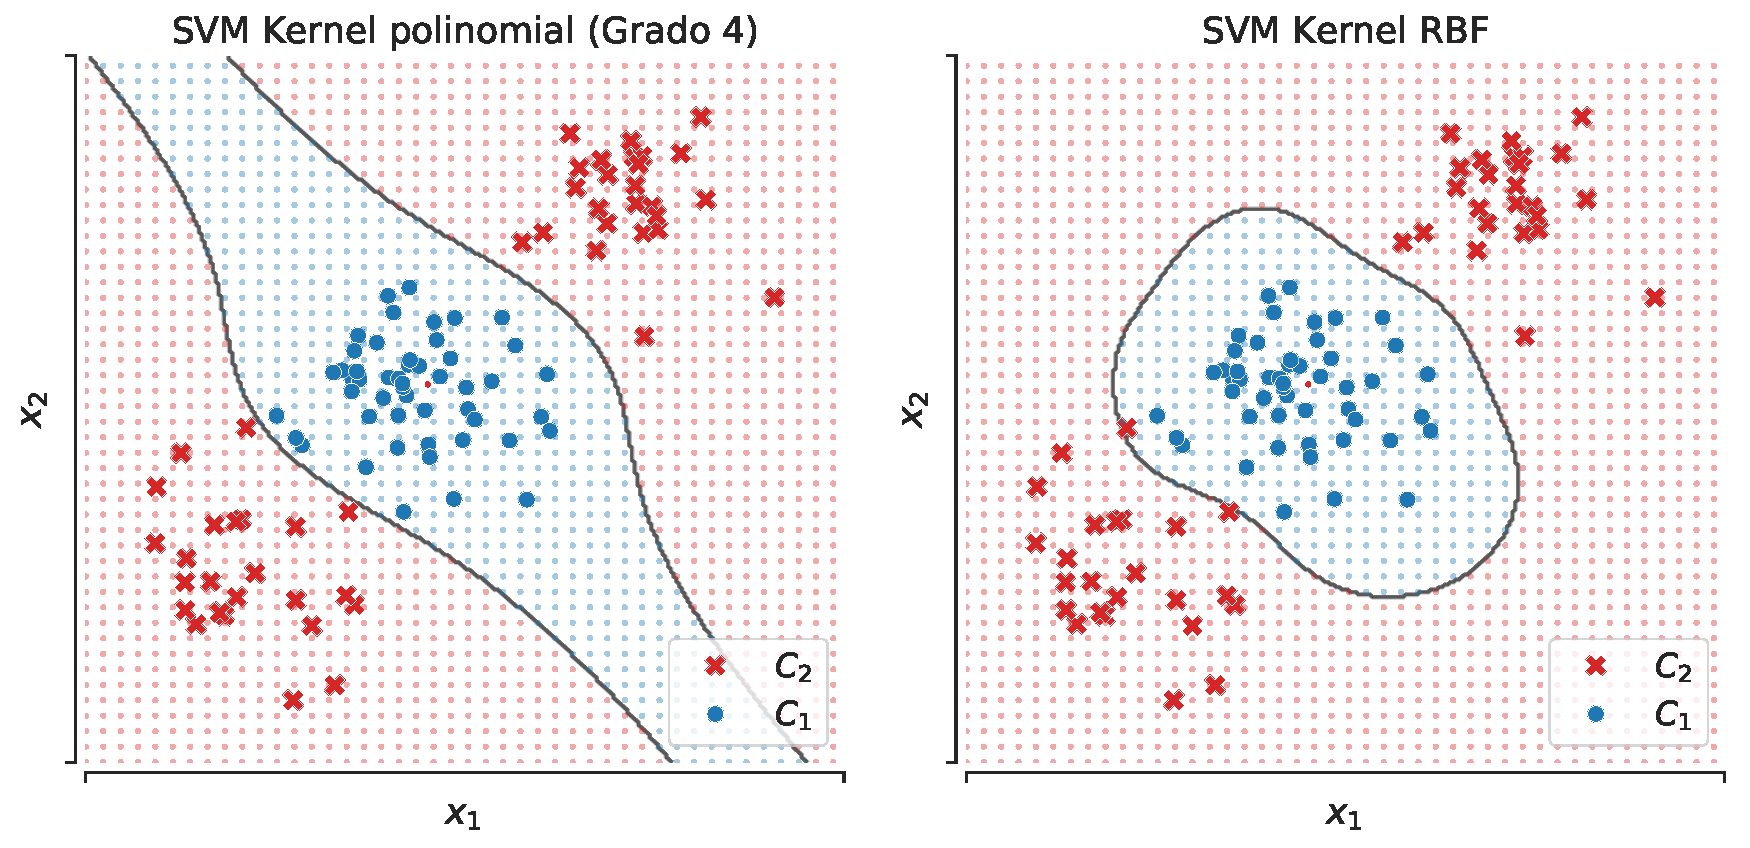
\includegraphics[width=0.75\textwidth]{img/cap5_svm_2kernels}
    \caption{Clasificación usando kernel SVM (margen suave) con distinto kernels: polinomial a la izquierda y RBF a la derecha.}
    \label{fig:ksvm}
\end{figure}

La Fig.~\ref{fig:ksvm}  muestra la implementación de kernel SVM para dos kernels: a la izquierda se ocupó un kernel polinomial de grado $3$, dicho kernel se caracteriza por su curvatura en los límites del clasificador, mientras que a la derecha se ocupó un kernel RBF, el cual es capaz de encontrar fronteras de decisión más curvadas (infinitamente diferenciables).\\

Finalmente, observemos que los métodos de kernel tienen una tremenda ventaja computacional con respecto a sus contrapartes sin kernel. Transformar los datos a un espacio de mayor dimensión  definiendo explícitamente $\phi(x)$ puede ser muy costoso, o incluso imposible, en el caso que el espacio de llegada sea infinito-dimensional. Usando kernels, por el contrario, dicha función queda implícita en el problema, y el método tiene un costo finito a pesar de que el modelo efectivamente opera en un espacio de características infinito (en el caso de RBF por ejemplo).


%-Comparar rendimiento de logistic regression c on SVM lineal
%-Usar diferentes Kernels
%-Ver el overfitting cuando ocupas un polinomio de muchos grados
%-Ver la importancia de escalar los datos

